\documentclass[a4paperpaper,9pt,twocolumn,twoside,printwatermark=false]{pinp}

%% Some pieces required from the pandoc template
\providecommand{\tightlist}{%
  \setlength{\itemsep}{0pt}\setlength{\parskip}{0pt}}

% Use the lineno option to display guide line numbers if required.
% Note that the use of elements such as single-column equations
% may affect the guide line number alignment.

\usepackage[T1]{fontenc}
\usepackage[utf8]{inputenc}

% The geometry package layout settings need to be set here...
\geometry{layoutsize={0.95588\paperwidth,0.98864\paperheight},%
          layouthoffset=0.02206\paperwidth,%
		  layoutvoffset=0.00568\paperheight}

\definecolor{pinpblue}{HTML}{185FAF}  % imagecolorpicker on blue for new R logo
\definecolor{pnasbluetext}{RGB}{101,0,0} %



\title{Wine Quality Analysis}

\author[]{Hirley Dayan Lourenço da Silva \emph{and} Marcia Maria Parmigiani
Martins}


\setcounter{secnumdepth}{0}

% Please give the surname of the lead author for the running footer
\leadauthor{}

% Keywords are not mandatory, but authors are strongly encouraged to provide them. If provided, please include two to five keywords, separated by the pipe symbol, e.g:
 \keywords{  Logistic Regression |  glm |  glmnet  }  

\begin{abstract}
Logistic regression is used to describe data and to explain the
relationship between one dependent binary variable and one or more
independent variables. This work explores Logistic Regression techniques
for creating a model for classifying the quality of wines based on a few
chemical features.
\end{abstract}

\dates{Unicamp Data Science - Supervised Learning Module}

% initially we use doi so keep for backwards compatibility
% new name is doi_footer


\begin{document}

% Optional adjustment to line up main text (after abstract) of first page with line numbers, when using both lineno and twocolumn options.
% You should only change this length when you've finalised the article contents.
\verticaladjustment{-2pt}

\maketitle
\thispagestyle{firststyle}
\ifthenelse{\boolean{shortarticle}}{\ifthenelse{\boolean{singlecolumn}}{\abscontentformatted}{\abscontent}}{}

% If your first paragraph (i.e. with the \dropcap) contains a list environment (quote, quotation, theorem, definition, enumerate, itemize...), the line after the list may have some extra indentation. If this is the case, add \parshape=0 to the end of the list environment.


\subsection{Introduction}\label{introduction}

This report contains an analysis of \textbf{WineQuality} datasets, using
a machine learning pipeline for exploring the datasets and proposing a
logistic classifier model for identifying good and bad wines based on a
few features.

\begin{figure}[h]
  \begin{center}
    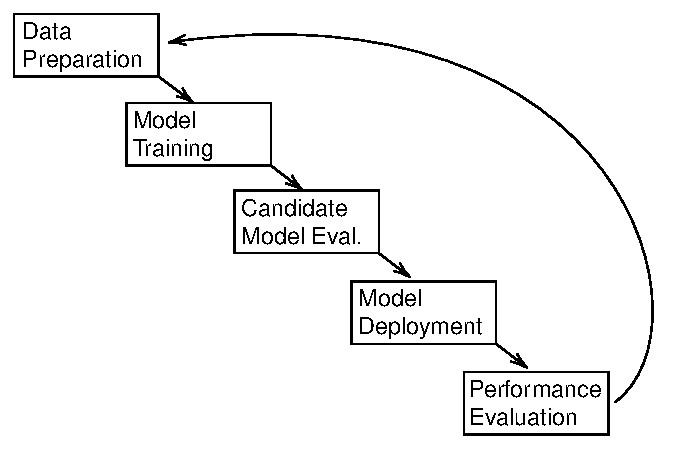
\includegraphics[width=0.45\textwidth, height=2.5in]{pipeline} 
  \caption{Machine Learning Pipeline}\label{fig}
  \end{center}
\end{figure}

\subsection{Data Preparation}\label{data-preparation}

There are \textbf{3898} samples in the \textbf{training} dataset and
\textbf{1299} samples in the \textbf{validation} dataset. The
\textbf{validation} dataset represents \textbf{25\%} of the total
available data (both \textbf{training} and \textbf{validation}
datasets). The \textbf{testing} dataset contains \textbf{1300} samples.
A few samples of the \textbf{training} dataset is shown in the
\textbf{Table \ref{tab:TrainingDataset}}.

\begin{table}[ht]
\begin{center}
\begin{tabular}{r|rrrrrr}
\hline
 & 1 & 2 & 3 & 4 & 5 & 6 \\
\hline
fixed.acidity & 7.10 & 6.00 & 7.90 & 6.20 & 7.00 & 7.00 \\
volatile.acidity & 0.33 & 0.39 & 0.18 & 0.28 & 0.50 & 0.31 \\
citric.acid & 0.30 & 0.17 & 0.49 & 0.51 & 0.25 & 0.31 \\
residual.sugar & 3.30 & 12.00 & 5.20 & 7.90 & 2.00 & 9.10 \\
chlorides & 0.03 & 0.05 & 0.05 & 0.06 & 0.07 & 0.04 \\
free.sulfur.dioxide & 30.00 & 65.00 & 36.00 & 49.00 & 3.00 & 45.00 \\
total.sulfur.dioxide & 102.00 & 246.00 & 157.00 & 206.00 & 22.00 & 140.00 \\
density & 0.99 & 1.00 & 1.00 & 1.00 & 1.00 & 0.99 \\
pH & 3.08 & 3.15 & 3.18 & 3.18 & 3.25 & 2.98 \\
sulphates & 0.31 & 0.38 & 0.48 & 0.52 & 0.63 & 0.31 \\
alcohol & 12.30 & 9.00 & 10.60 & 9.40 & 9.20 & 12.00 \\
quality & 1.00 & 0.00 & 0.00 & 0.00 & 0.00 & 1.00 \\
\hline
\end{tabular}
\caption{\label{tab:TrainingDataset}Training dataset}
\end{center}
\end{table}

\textbf{Training}, \textbf{validation} and \textbf{test} datasets
contains the following number of incomplete samples:

\begin{itemize}
\tightlist
\item
  \textbf{Training}: \textbf{0} incomplete samples
\item
  \textbf{Validation}: \textbf{0} incomplete samples
\item
  \textbf{Testing}: \textbf{0} incomplete samples
\end{itemize}

As shown above, there are \textbf{no} incomplete cases in the
\textbf{training}, \textbf{validation} and \textbf{testing} datasets.

\begin{table}[ht]
\begin{center}
\begin{tabular}{llllllllllllllllllllllllllllllllllllllllllllllllllllllllllllllllllllllll}
\hline
 & Min. & 1st Qu. & Median & Mean & 3rd Qu. & Max. \\
\hline
fixed.acidity & 3.80 & 6.40 & 6.90 & 7.19 & 7.60 & 15.90 \\
volatile.acidity & 0.08 & 0.23 & 0.29 & 0.34 & 0.40 & 1.58 \\
citric.acid & 0.00 & 0.24 & 0.31 & 0.32 & 0.39 & 1.66 \\
residual.sugar & 0.60 & 1.80 & 3.00 & 5.42 & 8.00 & 65.80 \\
chlorides & 0.01 & 0.04 & 0.05 & 0.06 & 0.06 & 0.61 \\
free.sulfur.dioxide & 1.00 & 17.00 & 29.00 & 30.64 & 41.00 & 146.50 \\
total.sulfur.dioxide & 6.00 & 76.25 & 118.00 & 115.33 & 155.00 & 366.50 \\
density & 0.99 & 0.99 & 0.99 & 0.99 & 1.00 & 1.04 \\
pH & 2.74 & 3.11 & 3.21 & 3.22 & 3.32 & 4.01 \\
sulphates & 0.23 & 0.43 & 0.51 & 0.53 & 0.60 & 2.00 \\
alcohol & 8.00 & 9.50 & 10.30 & 10.47 & 11.30 & 14.90 \\
quality & 0.00 & 0.00 & 0.00 & 0.20 & 0.00 & 1.00 \\
\hline
\end{tabular}
\caption{\label{tab:SummaryBeforeNormalization}Training dataset overview (without normalization)}
\end{center}
\end{table}

\textbf{Table \ref{tab:SummaryBeforeNormalization}} and \textbf{Table
\ref{tab:SummaryAfterNormalization}} present an overview of the
\textbf{training} dataset before and after normalization. For
normalizing the datasets it was used the \textbf{min}-\textbf{max}
normalization, as follows:

\begin{gather}
x'=\frac{x-min(x)}{max(x)-min(x)}
\end{gather}

\begin{table}[ht]
\begin{center}
\begin{tabular}{llllllllllllllllllllllllllllllllllllllllllllllllllllllllllllllllllllllll}
\hline
 & Min. & 1st Qu. & Median & Mean & 3rd Qu. & Max. \\
\hline
fixed.acidity & 0.00 & 0.21 & 0.26 & 0.28 & 0.31 & 1.00 \\
volatile.acidity & 0.00 & 0.10 & 0.14 & 0.17 & 0.21 & 1.00 \\
citric.acid & 0.00 & 0.14 & 0.19 & 0.19 & 0.23 & 1.00 \\
residual.sugar & 0.00 & 0.02 & 0.04 & 0.07 & 0.11 & 1.00 \\
chlorides & 0.00 & 0.04 & 0.06 & 0.07 & 0.09 & 1.00 \\
free.sulfur.dioxide & 0.00 & 0.11 & 0.19 & 0.20 & 0.27 & 1.00 \\
total.sulfur.dioxide & 0.00 & 0.19 & 0.31 & 0.30 & 0.41 & 1.00 \\
density & 0.00 & 0.10 & 0.15 & 0.15 & 0.19 & 1.00 \\
pH & 0.00 & 0.29 & 0.37 & 0.38 & 0.46 & 1.00 \\
sulphates & 0.00 & 0.11 & 0.16 & 0.17 & 0.21 & 1.00 \\
alcohol & 0.00 & 0.22 & 0.33 & 0.36 & 0.48 & 1.00 \\
quality & 0.00 & 0.00 & 0.00 & 0.20 & 0.00 & 1.00 \\
\hline
\end{tabular}
\caption{\label{tab:SummaryAfterNormalization}Training dataset overview (normalized)}
\end{center}
\end{table}

The box plot in the \textbf{Figure \ref{fig:DistribuitionAnalysis}}
gives a good overview of the data distribution of the \textbf{training}
dataset before the removal of the outliers. For the removal of the
outliers, which are values that differ considerably from the majority of
a set of data, different techniques are available. In this study,
outlier removal was performed using the \emph{capping} technique,by
replacing values outside the \(1.5*IQR\) limits, with the lower limit
replaced by the \textbf{5th} percentile and the bigger limit replaced by
the \textbf{95th} percentile.

\begin{figure}

{\centering 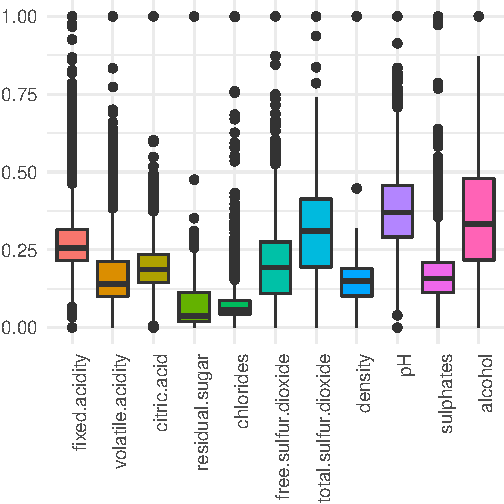
\includegraphics{WineQualityAnalysis_files/figure-latex/DistribuitionAnalysis-1} 

}

\caption{Data distribuition analysis}\label{fig:DistribuitionAnalysis}
\end{figure}

The lower and upper limits are calculated by the equations:

\begin{gather}
IQR = Q3 - Q1 \\ 
Lower = Q1 - 1.5 * IQR \\ 
Upper = Q3 + 1.5 * IQR
\end{gather}

Once the limits are calculated, outliers below the \textbf{5th}
percentile and above the \textbf{95th} percentile are replaced by both
\textbf{\emph{Lower}} and \textbf{\emph{Upper}} limits, respectively.

After the \textbf{capping} of the outliers, the new data distribution is
shown in \textbf{Figure \ref{fig:DistributionAnalysis2}}.

\begin{figure}

{\centering 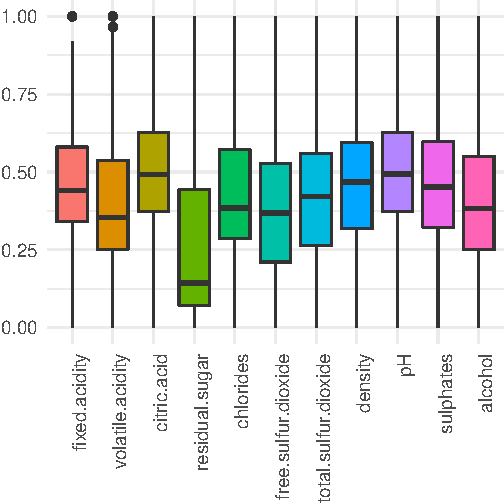
\includegraphics{WineQualityAnalysis_files/figure-latex/DistributionAnalysis2-1} 

}

\caption{Data distribuition analysis after capping}\label{fig:DistributionAnalysis2}
\end{figure}

According to the quality, the datasets are balanced as follows:

\begin{itemize}
\tightlist
\item
  \textbf{Tranining}: \textbf{19.78\%} of good wine samples
\item
  \textbf{Validation}: \textbf{64.36\%} of good wine samples
\item
  \textbf{Test}: \textbf{61.38\%} of good wine samples
\end{itemize}

\subsection{Model Training, Deployment and
Evaluation}\label{model-training-deployment-and-evaluation}

For training the model, quadratic and cubic functions were created with
the dataset features. Additionally, the \textbf{\emph{SMOTE}} technique
was used for dealing with the imbalanced datasets.

\begin{table}[ht]
\begin{center}
\begin{tabular}{r|rrr}
\hline
Formula & BACC & F1 & Good Wine Perc \\
\hline
1 & 0.7041 & 0.6721 & 66.67 \\
1 & 0.6836 & 0.5902 & 57.15 \\
2 & 0.7115 & 0.6804 & 66.67 \\
2 & 0.6894 & 0.5981 & 57.15 \\
2 & 0.6573 & 0.5199 & 50.00 \\
3 & 0.7246 & 0.6941 & 66.67 \\
3 & 0.6867 & 0.6054 & 57.15 \\
3 & 0.6692 & 0.5517 & 50.00 \\
\hline
\end{tabular}
\caption{\label{tab:CrossAnalysis}Cross analysis matrix (without penalty terms)}
\end{center}
\end{table}

For fitting the model, the \textbf{\texttt{glm}} function was used for
tuning the predefined functions, with the \textbf{training} dataset
re-balancing during validation. The result of the analysis can be found
in \textbf{Table \ref{tab:CrossAnalysis}}. The \textbf{confusion matrix}
of the predicted wine quality against the actual classification, when
using the \textbf{testing} dataset, can be found in the \textbf{Table
\ref{tab:ConfusionMatrix}}. The performance during the tests is also
shown by the \textbf{ROC} curve in \textbf{Figure \ref{fig:ROC1}}.

\begin{table}[ht]
\begin{center}
\begin{tabular}{rrrr}
\hline
 & 0 & 1 \\
\hline
0 & 464 & 450 \\
1 & 38 & 348 \\
\hline
\end{tabular}
\caption{\label{tab:ConfusionMatrix}Confusion matrix (without penalty terms)}
\end{center}
\end{table}

\begin{figure}

{\centering 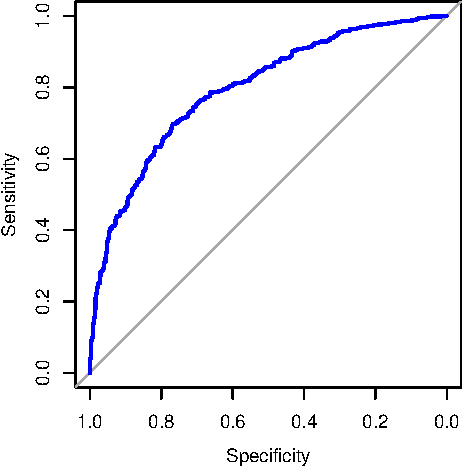
\includegraphics{WineQualityAnalysis_files/figure-latex/ROC1-1} 

}

\caption{ROC (without penalty terms)}\label{fig:ROC1}
\end{figure}

The function \textbf{\texttt{glmnet}} was also used for fitting the
model, and during the evaluation of the quadratic and cubic functions,
penalties were applied by changing the value of \textbf{\texttt{lambda}}
parameter. Similarly to the previous model fitting by
\textbf{\texttt{glm}}, the \textbf{training} dataset was also
re-balanced during the training. The result of that analysis can be
found in \textbf{Table \ref{tab:CrossAnalysis2}}. For avoiding spending
space in this report, the \textbf{Table \ref{tab:CrossAnalysis2}} does
not bring all collected values in the training. Only the values with
\textbf{Balanced Accuracy (BACC)} bigger than \textbf{70\%} are shown.
The \textbf{confusion matrix} for the predicted wine quality against the
actual quality, in the the \textbf{testing} dataset, can be found in
\textbf{Table \ref{tab:ConfusionMatrix2}}. The performance during the
tests of the classifier is also shown by the \textbf{ROC} curve in
\textbf{Figure \ref{fig:ROC2}}.

\begin{table}[ht]
\begin{center}
\begin{tabular}{r|rrrrr}
\hline
Formula & Alpha & Lambda & BACC & F1 & Good Wine Perc \\
\hline
1 & 0 & 0.0 & 0.7041 & 0.6721 & 66.67 \\
1 & 0 & 0.0 & 0.7041 & 0.6721 & 66.67 \\
1 & 0 & 0.0 & 0.7041 & 0.6721 & 66.67 \\
1 & 0 & 0.0 & 0.7041 & 0.6721 & 66.67 \\
1 & 0 & 0.0 & 0.7041 & 0.6721 & 66.67 \\
1 & 0 & 0.0 & 0.7063 & 0.6731 & 66.67 \\
1 & 0 & 0.0 & 0.7100 & 0.6804 & 66.67 \\
1 & 0 & 0.1 & 0.7160 & 0.7033 & 66.67 \\
2 & 0 & 0.0 & 0.7115 & 0.6804 & 66.67 \\
2 & 0 & 0.0 & 0.7115 & 0.6804 & 66.67 \\
2 & 0 & 0.0 & 0.7115 & 0.6804 & 66.67 \\
2 & 0 & 0.0 & 0.7115 & 0.6804 & 66.67 \\
2 & 0 & 0.0 & 0.7126 & 0.6809 & 66.67 \\
2 & 0 & 0.0 & 0.7127 & 0.6761 & 66.67 \\
2 & 0 & 0.0 & 0.7059 & 0.6687 & 66.67 \\
2 & 0 & 0.1 & 0.7131 & 0.6866 & 66.67 \\
3 & 0 & 0.0 & 0.7212 & 0.6911 & 66.67 \\
3 & 0 & 0.0 & 0.7212 & 0.6911 & 66.67 \\
3 & 0 & 0.0 & 0.7224 & 0.6930 & 66.67 \\
3 & 0 & 0.0 & 0.7192 & 0.6915 & 66.67 \\
3 & 0 & 0.0 & 0.7215 & 0.6878 & 66.67 \\
3 & 0 & 0.0 & 0.7160 & 0.6776 & 66.67 \\
3 & 0 & 0.0 & 0.7096 & 0.6697 & 66.67 \\
3 & 0 & 0.1 & 0.7121 & 0.6814 & 66.67 \\
3 & 0 & 1.0 & 0.7022 & 0.7282 & 66.67 \\
\hline
\end{tabular}
\caption{\label{tab:CrossAnalysis2}Cross analysis matrix (with penalty terms)}
\end{center}
\end{table}

\begin{table}[ht]
\begin{center}
\begin{tabular}{rrrr}
\hline
 & 0 & 1 \\
\hline
0 & 478 & 527 \\
1 & 24 & 271 \\
\hline
\end{tabular}
\caption{\label{tab:ConfusionMatrix2}Confision matrix (with penalty terms)}
\end{center}
\end{table}

\begin{figure}

{\centering 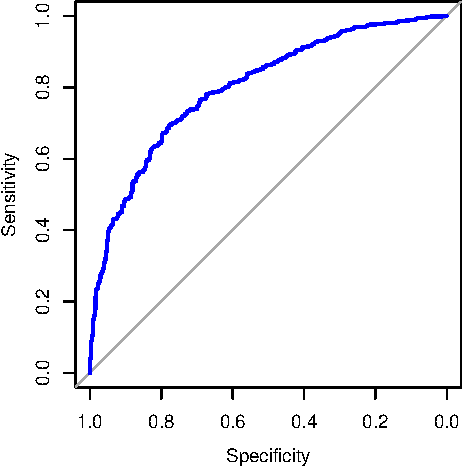
\includegraphics{WineQualityAnalysis_files/figure-latex/ROC2-1} 

}

\caption{ROC (with penalty terms)}\label{fig:ROC2}
\end{figure}

\subsection{Final Conclusions}\label{final-conclusions}

The logistic regression classifier with a generalized linear model with
penalization, by means of the function \textbf{\texttt{glmnet}}, has big
potential for bringing good results due to its fine-tuning parameters.
Despite all the potentials of the \textbf{\texttt{glmnet}}, this study
showed that the \textbf{\texttt{glm}} classifier performs well, giving
almost similar results as the \textbf{\texttt{glmnet}} classifier. The
dataset features were not enough for creating a good classifier, in both
cases evaluated, and the addition of 3rd-degree components was necessary
to increase the performance during training and validation.
Additionally, the tuning of the classifier with a different proportion
of wine classes showed that a better performance can be achieved by
having more good wine samples in the training dataset.

%\showmatmethods


\bibliography{bibliography}
\bibliographystyle{jss}



\end{document}

